The mathematical laws describing the deformation of a solid body are summarized in this section. First, the kinematic laws governing the motion of each material point belonging to a solid are considered. Then \textit{strain} measures are associated to internal forces through the thermodynamic framework so that \textit{constitutive equations} are derived. For a more exhaustive review of governing equations, see for instance \cite[Chapters~1-3]{Foundation_of_elasticity}, \cite{Truesdell}, \cite[Ch.7]{Simo}, \cite[Ch.3 \& 5]{Belytschko}.

\subsection{Kinematic laws -- Strain measures}
We consider a three-dimensional solid domain with volume denoted by $\Omega \subset \Rbb^3$ bounded by the surface $\partial \Omega$. This body undergoes external forces that can either be localized on a part of the external surface of the body (\textit{i.e. surface forces}) or act in the whole solid domain (\textit{i.e. volume forces}). Due to the presence of such sollicitations, the volume may change during a deformation within the time interval $\tau = \[0,T\]$ and will hence be written as a function of time $\Omega(t)$ ($t\in \tau$). The state of the solid at time $t=0$, corresponding to a non-deformed state with volume $\Omega(t=0)=\Omega_0$, is referred to as the \textit{initial configuration}. Some problems require the use of a \textit{reference configuration} that can be deformed and to which equations are referred. In what follows, the reference and initial conditions are identical. At a given time $t>0$, the volume $\Omega(t)=\Omega_t$ corresponds to the \textit{current configuration}. These configurations are depicted in figure \ref{fig:deformationFunction}.
\begin{figure}[h]
  \centering
  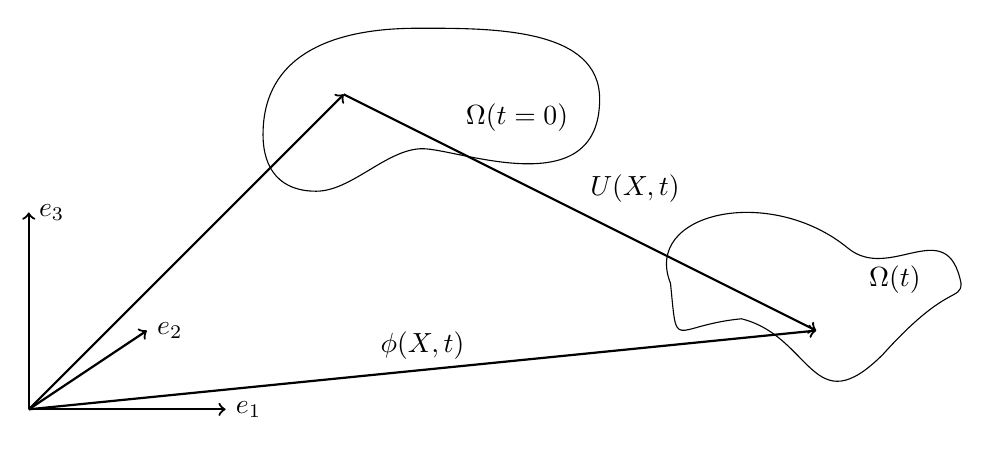
\begin{tikzpicture}
  %\draw[step=1.0,black,thin] (-3.,-1.) grid (3,4.);
  %\draw (-3,-1) -- (3,-1) -- (3,4) -- (-3,4) -- (-3,-1);
  \draw[thick,->] (-5,-2.5) -- (-2.5,-2.5) node [right] {$\vect{e}_1$};
  \draw[thick,->] (-5,-2.5) -- (-5,0.) node [right] {$\vect{e}_3$};
  \draw[thick,->] (-5,-2.5) -- (-3.5,-1.5) node [right] {$\vect{e}_2$};
  \begin{scope}[scale=0.45]
    \draw (-3,0.6) .. controls +(1,0) and +(-1,0) .. (0,1.8)  
    .. controls +(1,0) and +(0,-3) .. (5,3.2) 
    .. controls +(0,2) and +(2,0)  .. (0,5.2) 
    .. controls +(-1,0) and +(0,3) .. (-4.5,2.2) 
    .. controls +(0,-1) and +(-1,0).. (-3,0.6) ;
  \end{scope}
  \node at (1.2,1.2) {$\Omega(t=0)$};
  %% Deformed body +2.
  \begin{scope}[scale=0.9]
    \draw (0.+0.5+4.,0-1.5) ..controls (1.+0.5+4.,-0.25-1.5) and (1.+0.5+4.,-1.5-1.5) .. (2.+0.5+4.,-0.5-1.5) ..controls (2.9+0.5+4.,0.5-1.5) and (3.1+0.5+4.,0.25-1.5) .. (3.1+0.5+4.,0.5-1.5) ..controls (2.9+0.5+4.,1.5-1.5) and (2.1+0.5+4.,.5-1.5) .. (1.5+0.5+4.,1.-1.5) ..controls (0.4+0.5+4.,1.9-1.5) and (-1.4+0.5+4.,1.5-1.5) .. (-1.+0.5+4.,0.5-1.5)..controls (-0.4+0.+4.,-0.-2.) and (-1+0.5+4.,0.4-2.) .. (0+0.5+4.,0-1.5);
  \end{scope}
  \node at (6.,-0.85) {$\Omega(t)$};
  \draw[->,thick] (-5,-2.5) -- (-1.,1.5) node [midway,left] {$\X$};
  \draw[->,thick] (-5,-2.5) -- (5.,-1.5) node [midway,above] {$\vect{\phi}(\vect{X},t)$};
  \draw[->,thick] (-1.,1.5) -- (5.,-1.5) node [midway,above right] {$\vect{U}(\vect{X},t)$};
\end{tikzpicture}

%%% Local Variables:
%%% mode: latex
%%% TeX-master: "../../mainManuscript"
%%% End:
  \caption{Deformation of a solid body between a reference state $\Omega_0$ to a subsequent state $\Omega_t$.}
  \label{fig:deformationFunction}
\end{figure}

In the reference configuration, every material particle is located by their position vectors: $\vect{X}=X_\alpha \vect{e}_\alpha$, where $X_\alpha$ denotes the \textit{Lagrangian coordinates} and $\vect{e}_\alpha$ the basis vectors. At a subsequent time $t$, the particle initially located at $\vect{X}$ may have moved and its current location is given by the smooth mapping $\vect{\phi}(\vect{X},t)=\phi_i(\vect{X},t)\vect{e}_i$. Thus, the mapping $\vect{\phi}$ provides the paths of every particle of the solid during the deformation. In the lagrangian coordinates system, every particles are tracked during the deformation while the \textit{Eulerian coordinates}, denoted by $\vect{x}=x_i\vect{e}_i$, correspond to a \textit{spatial description}.
Note that in the above definitions Greek indices are used for quantities evaluated in the reference configuration whereas Latin ones refer to quantities defined in the current configuration. 

The \textit{displacement} and \textit{velocity} vectors of a particle between the reference and the current configuration are respectively:
\begin{align}
    &\vect{u}(\vect{X},t)=\vect{\phi}(\vect{X},t) - \vect{X} \qquad \forall\:\: \vect{X},t \in \Omega_0\times \tau  \label{eq:displacement}\\
    &\vect{v}(\vect{X},t)=\drond{\vect{\phi}}{t}(\vect{X},t) = \vect{\dot{\phi}}(\vect{X},t) \qquad  \forall\: \: \vect{X},t \in \Omega_0\times \tau  \label{eq:velocity}
\end{align}
where the superposed dot denotes the material time derivative. Then, the second-order two-point \textit{deformation gradient} tensor is defined as:
\begin{equation}
  \label{eq:F_phi}
    \tens{F}=\nablat_0 \vect{\phi} (\vect{X},t)
\end{equation}
where $\nablat_0 (\bullet)$ refers to the gradient operator on the reference configuration. This tensor can also be written by using equation \eqref{eq:displacement}:
\begin{equation}
  \tens{F}= \nablat_0 \vect{u}(\vect{X},t) + \tens{I} \label{eq:F_displacement}
\end{equation}
with $\tens{I}$, the second-order identity tensor. The deformation gradient tensor characterizes the variations of lengths, areas and volumes. Indeed, the infinitesimal vector, oriented surface and volume elements respectively denoted by $\vect{dX},\vect{dS}$ and $dV$ and defined in the reference configuration transorm respectively to:
\begin{equation}
  \label{eq:transport_equations}
  \begin{aligned}
    & dx_i=F_{i\alpha}dX_\alpha \\
    & ds_i=J F_{\alpha i}^{-1}dS_{\alpha} \\
    & dv=JdV 
  \end{aligned}
\end{equation}
in the current configuration. The transport equations \eqref{eq:transport_equations} involve the determinant of the deformation gradient $J=\det(\tens{F})>0$, also called the \textit{Jacobian of the deformation}. The deformation gradient is a strain measure since it accounts for changes in lengths and angles (\textit{i.e. the change of shape of a body}). Other strain measures can be used such as the \textit{right Cauchy-Green} or the \textit{Green-Lagrange} tensors, respectively defined as:
\begin{equation*}
   \tens{C}=\tens{F}^T\tens{F} \quad ; \quad \tens{E}=\frac{1}{2}(\tens{C}-\tens{I})
\end{equation*}
where $\tens{I}$ is the second-order identity tensor. The Green-Lagrange tensor can also be written by means of equation \eqref{eq:F_displacement}:
\begin{equation*}
  \tens{E}=\frac{1}{2}(\nablat_0 \vect{u} + \nablat_0 \vect{u}^T + \nablat_0 \vect{u}\nablat_0 \vect{u}^T)
\end{equation*}
In particular, when the deformation involves displacement vectors such that $\norm{\nablat_0 \vect{u}} \ll 1$, the last (second-order) term of the previous definition can be neglected leading to:
\begin{equation}
  \label{eq:epsilon}
  \tens{E} \approx \frac{1}{2}(\nablat_0 \vect{u} + \nablat_0 \vect{u}^T) = \tens{\eps}
\end{equation}
with $\tens{\eps}$ the \textit{linearized strain tensor}, the symmetric part of the displacement gradient. Such deformations fall in the \textit{linearized geometrical framework} or \textit{infinitesimal theory} and are characterized by small strain but possibly large displacements. Furthermore, when the deformation leads to a displacement vector $\norm{\vect{u}} \ll 1$ reference and current configurations are considered as indentical. These situations correspond to the \textit{small strain} framework for which the reference and current configurations are considered as identical.

\subsection{Balance equations}
In this section a solid domain $\Omega(t)$ undergoing a deformation is still considered within the time interval $\tau = \[0,T\]$. According to the formulation adopted in \cite{Plohr}, time derivatives of geometrical relations \eqref{eq:F_phi} and \eqref{eq:epsilon} combined to the definition of the velocity field \eqref{eq:velocity} yields kinematic conservations laws. Those conservation laws reads respectively:
\begin{align}
  & \tens{\dot{F}} - \nablat_0\vect{v} = \tens{0} \label{eq:HE_kinematic}\\
  & \tens{\dot{\eps}} - \nablat^s\vect{v} = \tens{0} \label{eq:HPP_kinematic}
\end{align}
where $\nablat^s$ denotes the symmetric gradient operator.

Then, we consider the conservation of mass in the continuum during the deformation in integral form:
\begin{equation*}
  \int_\Omega \rho d\Omega = \int_{\Omega_0} \rho_0 d\Omega \qquad \forall \: t \in  \tau
\end{equation*}
which, with the third transport formula reads:
\begin{equation}
  \label{eq:mass_conservation_law}
  \int_{\Omega_0} \(J\rho - \rho_0\) d\Omega = 0
\end{equation}
Leading to the first balance equation, namely the local conservation of mass:
\begin{equation}
  \label{eq:mass_balance}
  \rho = \frac{\rho_0}{J} \qquad \forall \: \vect{X},t \: \in \Omega_0\times \tau
\end{equation}
In particular, the linearised geometrical framework automatically satisfies this relation since current and reference configurations are the same (\textit{i.e.} $\rho=\rho_0 \: \forall t\in\tau$).

We now move on to the equilibrium between acceleration effects, namely \textit{intertia}, and external forces undergone by a solid $\Omega$. This conservation law corresponds to \textit{Newton's second law}:
\begin{equation*}
  \int_\Omega \rho \vect{\dot{v}} d\Omega = \int_{\partial \Omega} \vect{t} dS + \int_{\Omega} \rho\vect{b}d\Omega \qquad \forall \: t \in  \tau
\end{equation*}
where $\vect{t}$ denotes surface forces and $vect{b}$ volume forces in the current configuration. We then introduce the symmetric second-order \textit{Cauchy stress tensor} $\tens{\sigma}$ by using Cauchy's theorem $\vect{t}=\tens{\sigma}\cdot \vect{n}$ where $\vect{n}$ is the outwerd normal vector to the surface element $dS$. 

For further developments, the divergence theorem is required:
\begin{equation}
  \label{eq:Ostrogradski_th}
  \int_{\partial \Omega} (\bullet)\cdot \vect{dS}=\int_\Omega \nablav \cdot (\bullet) \: d\Omega
\end{equation}
where $\nablav \cdot (\bullet)$ denotes the divergence operator on the current configuration. Introduction of the previous formula in the second law of Newton leads to:
\begin{equation}
  \label{eq:Linear_momentum_conservation_eulerian}
  \int_{\Omega} \( \rho \vect{\dot{v}} - \nablav \cdot \tens{\sigma} -  \rho\vect{b} \) d\Omega = \vect{0} \qquad \forall \:t \in  \tau
\end{equation}
Conservation law \eqref{eq:Linear_momentum_conservation_eulerian} can be mapped to the reference configuration by using the transport formula of volume elements and the mass balance equation \eqref{eq:mass_balance}, thus yielding:
\begin{equation}
  \label{eq:Linear_momentum_conservation}
  \int_{\Omega_0} \( \rho_0 \vect{\dot{v}} - J \nablav \cdot \tens{\sigma} -  \rho_0\vect{b} \) d\Omega = \vect{0} \qquad \forall \: t \in\tau
\end{equation}
In equation \eqref{eq:Linear_momentum_conservation}, the divergence operator on the current configuration can be transported to the reference one by means of the \textit{Piola transform}:
\begin{definition}
  The Piola-Kirchhoff tranform $\tens{T}^P$ of a second-order tensor $\tens{T}$ is defined as:
  \begin{equation*}
    \tens{T}^P=J\tens{T}\cdot\tens{F}^{-1}
  \end{equation*}
  and satisfies:
  \begin{equation*}
    \nablav_0\cdot \tens{T}^P = J \nablav \cdot \tens{T}
  \end{equation*}
  where $\nablav_0\cdot (\bullet)$ is the divergence operator on the reference configuration.
\end{definition}
Another stress measure that corresponds to the Piola transform of Cauchy stress tensor is thus introduced, the \textit{first Piola-Kirchhoff stress tensor (PK1)} $\tens{\Pi}=J\tens{\sigma}\cdot\tens{F}^{-1}$. Hence, the vanishing of the integrand in equation \eqref{eq:Linear_momentum_conservation} yields the balance equation of the \textit{lagrangian linear momentum}:
\begin{equation}
  \label{eq:Lagrangian_linear_momentum}
  \rho_0 \vect{\dot{v}} - \nablav_0 \cdot \tens{\Pi} = \rho_0 \vect{b} \qquad \forall \: \: \vect{X},t \in \Omega_0 \times \tau 
\end{equation}
When considering deformations within the small strain framework the balance equation of linear momentum can be deduced from equation \eqref{eq:Linear_momentum_conservation_eulerian}, leading to:
\begin{equation}
  \label{eq:HPP_linear_momentum}
  \rho_0 \vect{\dot{v}} - \nablav \cdot \tens{\sigma} = \rho_0 \vect{b}  \qquad \forall \: \: \vect{x},t \in \Omega \times \tau 
\end{equation}

We complete the set of balance laws by considering the conservation of the energy of a system, also known as the \textit{first law of thermodynamics}. This law relates a balance between the rates of change of \textit{kinetic} and \textit{internal} energies, the power of external forces and the amount of heat entering the system as \textit{volume} or \textit{surface heat sources}.
\begin{equation*}
  \ddroit{}{t}\int_{\Omega} \(\frac{1}{2}\rho \vect{v}\cdot\vect{v} + \rho e\) d\Omega = \int_{\partial \Omega} \(\tens{\sigma}\cdot\vect{n}\)\cdot\vect{v} \: dS + \int_{\Omega} \rho\vect{b}\cdot\vect{v} \: d\Omega + \int_{\Omega} \rho r \:d\Omega - \int_{\partial \Omega} \vect{q}\cdot\vect{n} \: dS \qquad \forall \: t \in  \tau 
\end{equation*}
where $\vect{q}$ is the outward heat flux vector and $r$ is a volume heat source. By using the divergence theorem \eqref{eq:Ostrogradski_th}, the previous equation reads:
\begin{equation*}
\ddroit{}{t}\int_{\Omega} \(\frac{1}{2}\rho \vect{v}\cdot\vect{v} + \rho e\) d\Omega = \int_{\Omega} \(\nablav\cdot(\tens{\sigma}\cdot\vect{v}) +  \rho\vect{b}\cdot\vect{v} \) d\Omega + \int_{\Omega} \rho r \: d\Omega  - \int_{\partial \Omega} \vect{q}\cdot\vect{n} \: dS \qquad \forall \: t \in  \tau 
\end{equation*}
The transport of this relation on the reference configuration based on \eqref{eq:transport_equations} allows to introduce the time derivative of the left-hand side in the integral
\begin{equation*}
\int_{\Omega_0} \(\rho_0 \vect{\dot{v}} + \rho_0 \dot{e}\) d\Omega = \int_{\Omega_0} \(J\nablav\cdot(\tens{\sigma}\cdot\vect{v}) +  \rho_0\vect{b}\cdot\vect{v} \) d\Omega + \int_{\Omega_0} \rho_0 r \:d\Omega- \int_{\partial \Omega_0} J\vect{q}\cdot \tens{F}^{-1}\cdot\vect{n} \: dS \qquad \forall \: t \in  \tau 
\end{equation*}
Then, substitution of the linear momentum according to equation \eqref{eq:Lagrangian_linear_momentum} yields, after some algebra, the conservation law of internal energy:
\begin{equation}
  \label{eq:conservation_law_energy}
  \int_{\Omega_0} \rho_0 \dot{e} d\Omega = \int_{\Omega_0} \tens{\Pi}:\nablat_0\vect{v}\: d\Omega + \int_{\Omega_0} \(\rho_0r  - \nablav_0 \cdot \vect{Q}\) d\Omega \qquad \forall \: t \in  \tau 
\end{equation}
where $\vect{Q}=J\vect{q}\cdot \tens{F}^{-1}$ is the lagrangian heat flux vector. We thus deduce the balance equation of internal energy on the reference configuration:
\begin{equation}
  \label{eq:energy_balance}
  \rho_0 \dot{e} -  \tens{\Pi}:\nablat_0\vect{v}  + \nablav_0 \cdot \vect{Q}  = \rho_0 r \qquad \forall \: \: \vect{X},t \in \Omega_0 \times \tau 
\end{equation}
where $\nablat_0\vect{v} = \tens{\dot{F}}$. Finally, the small strain version of equation \eqref{eq:energy_balance} is: 
\begin{equation}
  \label{eq:energy_balance_euler}
  \rho_0 \dot{e} -  \tens{\sigma}:\nablat^{s} \vect{v}  + \nablav \cdot \vect{q}  = \rho_0 r \qquad \forall \: \: \vect{x},t \in \Omega \times \tau 
\end{equation}
in which $\nablat^{s} (\bullet)$ denotes the symmetric part of the gradient, in particular: $\nablat^s \vect{v} = \tens{\dot{\eps}}$. Stress measures are conjugate to strain measures through the power. In what follows, stress and strain may respectively be refered to as \textit{thermodynamic forces} and \textit{internal variables} according to the thermodynamics framework. The former obey a \textit{state equation} while the latter describe the evolution of the thermodynamic system. 
\subsection{Constitutive equations -- Thermodynamics}
The closure of a problem is given by the constitutive equations (\textit{i.e state laws}) for the stress. Once and for all, we consider here constitutive models within the \textit{Generalized Standard Materials} (GSM) framework \cite{GSM}.

\subsubsection*{The general (hyper)elasticity formulation}
First, the \textit{Clausius-Duhem} inequality resulting from combination of first and second laws of thermodynamics, reads: 
\begin{equation}
  \label{eq:Clausius-Duhem}
  \underbrace{\phantom{\frac{1}{\theta}} \tens{\Pi}:\tens{\dot{F}} + \rho_0 \(\theta \dot{\eta} -\dot{e}\)}_{\Dscr^{int}} \:-\:  \underbrace{\frac{1}{\theta} \vect{q} \cdot \nablav_0 \theta}_{-\Dscr^{th}} \geq 0  \qquad \forall \: \: \vect{X},t \in \Omega_0 \times \tau 
\end{equation}
where $\Dscr^{int}$ and $\Dscr^{th}$ are respectively the specific mechanical and thermal dissipations. Equation \eqref{eq:Clausius-Duhem} results in vanishing dissipations for \textit{reversible} processes and in a strict inequality for \textit{irreversible} ones. Furthermore, a widely used assumption consists in considering that the mechanical and thermal dissipations simultaneously satisfy non-negativeness. Note that the \textit{Fourier's law} of conduction is based on the non-negativeness of the thermal dissipation and leads to the following definition of the heat flux vector in order to ensure the positivity of the thermal dissipation:
\begin{equation*}
  \label{eq:Fourier_law}
  \vect{q}=-\tens{k}\cdot\nablav_0 \theta
\end{equation*}


The internal energy density is a function of strain, \textit{entropy} $\eta$ and additional state variables $\Vc_p, \: (1\leq p \leq N)$ describing irreversible processes. Recall that calligraphic symbols denote column array. It is more convenient to use its \textit{Legendre transform}, the \textit{Helmholtz free energy density potential} $\psi\(\tens{F},\theta,\Vcb\)=e\(\tens{F},\eta,\Vcb\)-\theta \eta$ where $\theta$ is the temperature. The free energy density is supposed \textit{objective} or \textit{frame indifferent} \cite[p.255]{Simo}, concave with respect to temperature and convex with respect to other variables. The mechanical dissipation can then be rewritten as:
\begin{equation*}
  \Dscr^{int} = \tens{\Pi}:\tens{\dot{F}} - \rho_0 \(\dot{\psi} +\eta \dot{\theta}\) 
\end{equation*}
The time derivative of Helmholtz free energy density:
\begin{equation}
  \label{eq:derivative_psi}
  \dot{\psi} = \drond{\psi}{\tens{F}}:\tens{\dot{F}} + \drond{\psi}{\theta}\dot{\theta} + \drond{\psi}{\Vcb}\dot{\Vcb}
\end{equation}
can be introduced within the mechanical dissipation so that one gets:
\begin{equation}
  \label{eq:Dint_psi_factor}
  \Dscr^{int} = \(\tens{\Pi}- \rho_0 \drond{\psi}{\tens{F}} \):\tens{\dot{F}} - \rho_0 \(\drond{\psi}{\theta} +\eta\) \dot{\theta}  - \rho_0\drond{\psi}{\Vcb}\dot{\Vcb} 
\end{equation}


Since the mechanical dissipation must be non-negative regardless of the nature of the deformation, it must in particular vanish for a reversible isothermal process (\textit{i.e. $\theta=const$}) for which every additional internal variables are constant. With these considerations, we are left with the relation:
\begin{equation*}
  \( \tens{\Pi} - \rho_0\drond{\psi}{\tens{F}} \): \tens{\dot{F}} = 0
\end{equation*}
holding regardless of the deformation, and hence:
\begin{equation}
  \label{eq:PK1_definition}
  \rho_0\drond{\psi}{\tens{F}} = \tens{\Pi}
\end{equation}
A material is said \textit{hyperelastic} if there exist a \textit{stored energy function} $\rho_0\psi$ from which can be derived the first Piola-Kirchhoff stress tensor \cite[p.8]{Foundation_of_elasticity}. The time derivative of this relation leads to:
\begin{equation}
  \label{eq:HE_tangent}
  \tens{\dot{\Pi}} = \rho_0\ddrond{\psi}{\tens{F}}{\tens{F}}:\tens{\dot{F}} = \Hbb:\tens{\dot{F}} 
\end{equation}
where $\Hbb$ is the $4$th order \textit{tangent modulus} tensor. Equivalently we have for linear elasticity:
\begin{equation}
  \label{eq:Cauchy_definition}
  \rho_0 \drond{\psi}{\tens{\eps}} = \tens{\sigma}
\end{equation}
and:
\begin{equation}
  \label{eq:HPP_tangent}
  \tens{\dot{\sigma}} = \rho_0\ddrond{\psi}{\tens{\eps}}{\tens{\eps}}:\tens{\dot{\eps}} = \Cbb:\tens{\dot{\eps}} 
\end{equation}
In equation \eqref{eq:HPP_tangent}, $\Cbb$ is the $4$th order \textit{elastic stiffness} tensor which has major and minor symmetries. For isotropic elasticity, $C_{ijkl}=\lambda \delta_{ij}\delta_{kl} + \mu \(\delta_{ik}\delta_{jl}+\delta_{il}\delta_{jk}\)$ yields \textit{Hook's law} with $(\lambda,\mu)$ are Lamé parameters.

Similar considerations lead to the state laws for entropy and for additional thermodynamic forces :
\begin{equation}
  \label{eq:thermodynamic_forces}
  \drond{\psi}{\theta} = - \eta \quad ; \quad \rho_0\drond{\psi}{\Vcb}=\Acb
\end{equation}
where $\Acb$ are thermodynamic forces associated to internal variables $\Vcb$.
In what follows, we shall consider hyperelastic or linear elastic deformations that do not involve irreversible processes (\textit{e.g. damage or thermal softening}). Hence, additional internal variables and associated thermodynamic forces are not activated in such situations. However, the cases of \textit{elastoplasticity} and \textit{elasto-viscoplasticity}, involving such variables and forces, will be considered in the linearized geometrical framework.

\begin{remark}
  \label{rq:isothermal_deformation}
  Temperature has been introduced as an internal variable and requires the introduction of the heat equation for the closure of the system:
  \begin{equation*}
    \rho_0 C \dot{\theta} = \rho_0 r - \nablav_0 \cdot \vect{Q} - \rho_0 \drond{\psi}{\Vcb}\dot{\Vcb} + \theta \(\drond{\tens{\Pi}}{\theta}:\tens{\dot{F}} - \drond{\Acb}{\theta}\dot{\Vcb} \)
  \end{equation*}
  Nevertheless, we will restrict our attention in the following to isothermal deformation so that temperature can be omitted and internal energy balance equation \eqref{eq:energy_balance} or \eqref{eq:energy_balance_euler} is automatically satisfied. Indeed, for isothermal processes the heat equation leads to:
  \begin{equation*}
    \rho_0 r - \nablav_0 \cdot \vect{Q} = \rho_0 \drond{\psi}{\Vcb}\dot{\Vcb}
  \end{equation*}
  which, once introduced in the energy balance \eqref{eq:energy_balance} yields:
  \begin{equation*}
    \rho_0 \dot{e} - \tens{\Pi}:\tens{\dot{F}} = \rho_0 \drond{\psi}{\Vcb}\dot{\Vcb}
  \end{equation*}
  By using the free energy density time derivative \eqref{eq:derivative_psi} and noting that $\eta=-\drond{\psi}{\theta} =0$, we get that each side of the previous equation vanishes.
\end{remark}


\subsubsection*{History-dependent models in small strain}
While elasticity does not involve dissipation, plasticity is characterized by irreversible strain and hardening variables $\Vcb$ that account for the loading history undergone by every material particles. Within the linearized geometrical framework, the infinitesimal strain tensor $\tens{\eps}$ is assume to be additively decomposed into an elastic and a plastic part:
\begin{equation}
  \label{eq:additive_plast}
  \tens{\eps} = \tens{\eps}^e + \tens{\eps}^p
\end{equation}
such that the mechanical dissipation only involve the plastic part:
\begin{equation}
  \label{eq:HPP_dissipation}
  \Dscr^{int}=\tens{\sigma}:\tens{\dot{\eps}}^p -\rho_0 \drond{\psi}{\Vcb}\dot{\Vcb} \geq 0
\end{equation}

A \textit{yield condition} is defined with the \textit{yield function} $f(\tens{\sigma},\Acb)$ so that that the elastic domain $\Ebb$ in stress space $(\tens{\sigma},\Acb)$ corresponds to:
\begin{equation}
  \label{eq:elastic_convex}
  \Ebb = \{ (\tens{\sigma},\Acb)\: | \: f(\tens{\sigma},\Acb) \leq 0\}
\end{equation}
According to the GSM framework \cite{GSM} we assume the existence of a dissipation pseudo-potential $\Phi(\tens{\sigma},\Vcb)$, convex with respect to thermodynamic forces and vanishing at the origin of the $(\tens{\sigma},\Vcb)$ space. This pseudo-potential enables the derivation of the plastic \textit{flow} and \textit{hardening} rules:
\begin{subequations}
  \begin{alignat}{2}
    \label{eq:flow_rule_plast}
     \tens{\dot{\eps}}^p&=&&\drond{\Phi}{f}\drond{f}{\tens{\sigma}}\\
    \label{eq:hardening_rule_plast}
     \dot{\Vcb}& = -&&\drond{\Phi}{f}\drond{f}{\Acb}
  \end{alignat}
\end{subequations}
where $\drond{\Phi}{f}=\dot{p}$ is the \textit{plastic multiplier}. We then distinguish two cases:
\begin{itemize}
\item \textbf{Rate-independent} plasticity is based on the assumption that admissible thermodynamic forces lie within the elastic domain \eqref{eq:elastic_convex}. The plastic multiplier is used as a Lagrange multiplier in order to ensure $f(\tens{\sigma},\Acb)\leq 0$ and must obey the \textit{K{\"u}hn-Tucker compatibility conditions}:
\begin{equation}
  \label{eq:Kuhn_Tucker}
  \dot{p} \geq 0 \quad ; \quad f \leq 0 \quad ; \quad \dot{p}f =0 
\end{equation}
The plastic multiplier, or the \textit{equivalent plastic strain rate} is determined by the \textit{consistency condition}:
\begin{equation}
  \label{eq:consistency_condition}
  \dot{f}=0
\end{equation}

% In analogy with the elastic law \eqref{eq:HPP_tangent}, rate-independent plastic evolutions are governed by the \textit{elastoplastic tangent modulus}:
% \begin{equation}
%   \label{eq:HPP_tangent_plasticity}
%   \tens{\dot{\sigma}}=\Cbb^{ep}:\tens{\dot{\eps}}
% \end{equation}

\item \textbf{Viscoplasticity} or \textbf{rate-dependent} plasticity can be seen as a regularization of rate-independent plasticity that relaxes the condition $f(\tens{\sigma},\Acb)\leq 0$ and thus leads to admissible thermodynamic forces outside the elastic domain \cite[p.58]{Simo}. Furthermore, the plastic fluxes $\tens{\dot{\eps}}^p, \dot{\Vcb}$ are completely determined by the knowlegde of the dissipation pseudo-potential. 
\end{itemize}
\subsubsection*{Examples of constitutive laws}
We now specify the above discussion to constitutive models that will be used in the following of the manuscript.

$\newline$
\textbf{The neo-Hookean hyperelastic model} is well-suited to describe rubber-like materials and is based on the polyconvex stored energy function:
\begin{equation}
  \label{eq:neo-hook_energy}
  \rho_0 \psi(J,\tens{F})= \frac{\kappa}{2}(J-1)^2 + \frac{\mu}{2}\[J^{-2/3} (\tens{F}:\tens{F})-3 \]
\end{equation}
where $\kappa$ is the bulk modulus and $\mu$ the Lam\'e shear modulus. We then introduce the \textit{tensor cross product} \cite{cross_tensor_product} of two second order two-point tensors $\tens{a}$ and $\tens{c}$, defined as:
\begin{equation}
  \label{eq:cross_tensor_product}
  \(\tens{a} \tens{\times} \tens{c}\)_{i\alpha}= \Ec_{ijk} \Ec_{\alpha \beta \gamma} a_{j\beta}b_{k\gamma}
\end{equation}
where $\Ec_{ijk}$ is the \textit{Levi-Civita} permutation symbol. By making use of this operator, the Jacobian $J$ can be written:
\begin{equation*}
  J=\frac{1}{6}\(\tens{F}\ttimes\tens{F}\):\tens{F}
\end{equation*}
or equivalently 
\begin{equation*}
  J=\frac{1}{3}\tens{H}:\tens{F}
\end{equation*}
in which $\tens{H}=\frac{1}{3}\tens{F}\ttimes\tens{F}=J\tens{F}^{-T}$ is the \textit{adjoint tensor} of the deformation gradient. Note that by using the tensor cross product operator, one can easily show that $\drond{J}{\tens{F}}=\tens{H}$. With these definitions, the derivative of the stored energy function \eqref{eq:neo-hook_energy} with respect to the deformation gradient can be computed so that the PK1 tensor can be derived:
\begin{equation}
  \label{eq:PK1_neo-hook}
  \tens{\Pi} = \mu J^{-2/3} \[\tens{F}- \frac{1}{3}\(\tens{F}:\tens{F}\) \tens{F}^{-T}\] + \kappa \(J-1\)\tens{H}
\end{equation}

The acoustic tensor $A_{ij}=N_\alpha H_{i\alpha j\beta} N_\beta$ for the neo-Hookean hyperelastic model is \cite{Haider_FVM}:
\begin{equation}
  \label{eq:neo-hook_acoustic}
  \begin{split}
      \tens{A}=\[\frac{5}{9}\mu J^{-8/3}\(\tens{F}:\tens{F}\)   + \kappa \]&(\tens{H}\cdot\vect{N})\otimes\(\tens{H}\cdot\vect{N} \)  + \mu J^{-2/3} \tens{I}  \\ &-\frac{2}{3}\mu J^{-5/3}\[(\tens{H}\cdot\vect{N})\otimes\(\tens{F}\cdot\vect{N} \)	+  (\tens{F}\cdot\vect{N})\otimes\(\tens{H}\cdot\vect{N} \)\]
  \end{split}
\end{equation}
The polyconvexity of this model ensures the positive definiteness of the acoustic tensor \eqref{eq:neo-hook_acoustic} \cite{Kluth}.

$\newline$
\textbf{The Saint-Venant-Kirchhoff hyperelastic model} is an extension of linear elastic Hook's law to hyperelasticity with a stored energy function that takes the form:
\begin{equation}
  \label{eq:SVK_energy}
  \rho_0\psi=\frac{1}{8}\(\tens{F}^T\tens{F}- \tens{I}\):\Cbb:\(\tens{F}^T\tens{F}- \tens{I}\)
\end{equation}
where $\Cbb$ is the elasticity tensor. In a similar manner as for the neo-Hookean model, the expression of the PK1 tensor is:
\begin{equation}
  \label{eq:SVK_PK1}
  \tens{\Pi} = \frac{1}{2}\lambda \(\tens{F}:\tens{F}- 3\) \tens{F} + \mu\tens{F}\(\tens{F}^T\tens{F}- \tens{I}\)
\end{equation}
The tangent modulus is then obtained by deriving this stress tensor:
\begin{equation}
  \label{eq:SVK_tangent}
  \Hbb = \lambda \[\tens{F}\otimes\tens{F} + \frac{1}{2} (\tens{F}:\tens{F}- 3)\Ibb\]+ \mu\(\Abb- \Ibb \)
\end{equation}
with $A_{i\alpha j \beta}=F_{k\alpha}F_{k\beta}\delta_{ij} + F_{j\alpha}F_{i\beta} +F_{i\mu} F_{j\mu}\delta_{\alpha\beta}$ and the fourth order identity tensor $I_{i\alpha j \beta}=\delta_{ij}\delta_{\alpha \beta}$. The previous tangent modulus finally leads to the acoustic tensor:
\begin{equation}
  \label{eq:SVK_acoustic}
  \begin{split}
    \tens{A} = \lambda \[\vphantom{\frac{1}{2}} (\tens{F}\cdot\vect{N})\otimes(\tens{F}\cdot\vect{N}) \right.+ &\left.\frac{1}{2} (\tens{F}:\tens{F}- 3)\tens{I}\] \\
    + & \mu\[(\tens{F}\cdot\vect{N})\cdot(\tens{F}\cdot\vect{N})\tens{I} + (\tens{F}\cdot\vect{N})\otimes(\tens{F}\cdot\vect{N}) + \tens{F}\cdot\tens{F}^T- \tens{I} \]
  \end{split}
\end{equation}
Even though it is known that this model can lead to non-physical solutions for very large deformation, it will be used for a one-dimensional strain problem for it enables to easily develop an analytical solution.  


$\newline$
\textbf{The plastic $J_2$ flow theory}, generally used to model metals, involves a yield function $f$ based on the second invariant of Cauchy stress deviatoric part $J_2=\tens{s}:\tens{s}$, where $\tens{s}=\tens{\sigma}-\frac{1}{3}\tr \tens{\sigma}$.
By considering internal variables and associated forces as: $\{\Vcb,\Acb\}=\{\[\tens{\eps}^p,p\],\[\tens{s}-\tens{Y},-R(p)\]\}$, one defines the following Helmoltz free energy density:
%can describe \textit{isotropic} linear hardening by setting $\tens{Y}=\tens{0}$, and \textit{kinematic} linear hardening with $R(p)=0$.The Helmoltz free energy density here reads:
\begin{equation}
  \label{eq:EP_helmoltz}
  \rho \psi = \frac{1}{2}\tens{\eps}^e:\Cbb:\tens{\eps}^e + \frac{2}{3}C\tens{\eps}^p:\tens{\eps}^p + H(r)
\end{equation}
In this expression, $r$ is to be defined, $H''(r)$ is the \textit{isotropic hardening} modulus and $\tens{Y}$ describes the evolution of the elastic domain center in stress deviator space and is related to \textit{kinematic hardening}. Linear hardenings will be considered here by setting either $\tens{Y}=\tens{0}$ for isotropic or $R(r)=0$ for kinematic hardening. The definition of thermodynamic forces \eqref{eq:thermodynamic_forces} leads to:
\begin{subequations}
  \begin{alignat}{1}
    \label{eq:eta}
    \tens{Y}&=\frac{2}{3}C\tens{\eps}^p \\
    \label{eq:isotropic_hardening}
    R &=H'(r)
  \end{alignat}
\end{subequations}
Furthermore, the \textit{von-Mises yield surface} is defined as:
\begin{equation}
  \label{eq:von-Mises_yield}
  f\(\tens{\sigma},\Acb \)= \sqrt{\frac{3}{2}}\norm{\tens{s}-\tens{Y}} - \(R(r)+\sigma^y\) \equiv 0
\end{equation}
$\sigma^y$ being the traction yield stress. The specialization of flow rules \eqref{eq:flow_rule_plast},\eqref{eq:hardening_rule_plast} leads to:
\begin{subequations}
  \begin{alignat}{1}
    \label{eq:plastic_strain_rate}
    &\tens{\dot{\eps}}^p=\dot{p}\sqrt{\frac{3}{2}}\frac{\tens{s}-\tens{Y}}{\norm{\tens{s}-\tens{Y}}}=\dot{p}\:\sqrt{\frac{3}{2}}\tens{m} \\
    \label{eq:equiv_plastic_strain_rate}
    &\dot{r}=\dot{p}
  \end{alignat}
\end{subequations}
where $r$ is identified from \eqref{eq:equiv_plastic_strain_rate} as the equivalent plastic strain. Considering rate-independent plasticity and combining the elastic law $\tens{\dot{\sigma}}=\Cbb:\(\tens{\dot{\eps}}-\tens{\dot{\eps}}^p\)$ yields the following evolution law:
\begin{equation}
  \label{eq:p_evolution}
  \dot{p}=\sqrt{\frac{3}{2}}\frac{2\mu}{3\mu+\beta}\tens{m}:\tens{\dot{\eps}}
\end{equation}
where $\beta=C$ for kinematic hardening and $\beta=R'(p)$ for isotropic hardening. Finally, equations \eqref{eq:plastic_strain_rate} and \eqref{eq:p_evolution}can be sequencially introduced in the elastic law so that one gets \cite[eq (2.2.22)]{Simo}:
\begin{equation}
  \label{eq:elastoplastic_tangent}
  \tens{\dot{\sigma}}=\(\Cbb - \frac{6\mu^2}{3\mu +\beta}\tens{m}\otimes\tens{m} \):\tens{\dot{\eps}} = \Cbb^{ep}:\tens{\dot{\eps}}
\end{equation}
with $\Cbb^{ep}$ the \textit{elastoplastic tangent modulus}. Note that (positive) linear hardenings ensure the positive definiteness of the elastoplastic acoustic tensor $\tens{A}^{ep}=\tens{A}^{elast} -  \frac{6\mu^2}{3\mu +\beta} (\tens{m}\cdot{n})\otimes(\tens{m}\cdot{n})$.  

Viscoplasticity on the other hand, leads to an explicit definition of the equivalent plastic strain:
\begin{equation}
  \label{eq:EVP_creep_law}
  \dot{p}=\left\langle \frac{f}{\eta}\right\rangle^n
\end{equation}
where $\left\langle\bullet\right\rangle=\frac{\bullet + \abs{\bullet}}{2}$ is the positive part function, and $n$ and $\eta$ are parameters arrising from the relaxation of the condition $f\leq 0$. Hence, rate-dependent plasticity is driven by the elastic law in which $\tens{\dot{\eps}^p}$ is given by \eqref{eq:flow_rule_plast} and \eqref{eq:EVP_creep_law}. 

\subsection{The general formulation}
We now summarize the conservation and constitutive laws obtained previously. Recall that the deformations considered here are isothermal and that history-dependent materials will be taken into account within linearized geometrical framework only. 
\subsubsection*{Linear elasticity and elasto-viscoplasticity}
We first gather the governing equations of elasticity and elasto-viscoplasticity within the linearized geometrical framework namely, the elastic law \eqref{eq:HPP_tangent}, the balance equation of linear momentum \eqref{eq:HPP_linear_momentum} and the kinematic law \eqref{eq:HPP_kinematic} which are repeated here for convenience:
\begin{align*}
  & \rho_0 \vect{\dot{v}} - \nablav \cdot \tens{\sigma} = \rho_0 \vect{b} \\
  & \tens{\dot{\sigma}} - \Cbb :\(\tens{\dot{\eps}}-\tens{\dot{\eps}}^p\) =\tens{0}\\
  & \tens{\dot{\eps}}-\nablat^s \vect{v} =\tens{0} \quad \qquad \forall \: \: \vect{x},t \in \Omega \times \tau 
\end{align*}
Note that the gradient operator of a vector $\vect{a}$ can be rewritten as a divergence operator:
\begin{equation}
  \label{eq:grad_div}
  \nablat \vect{a} = \nablav \cdot \(\vect{a}\otimes\tens{I} \)
\end{equation}
Hence, introduction of kinematic laws in the linear momentum balance yields, by assuming a cartesian coordinates system, the following \textit{conservative form}:
\begin{equation}
  \label{eq:general_conservative}
  \Qcb_t + \sum_{i=1}^D \drond{\Fcb\cdot \vect{e}_i}{x_i} = \Scb
\end{equation}
where the vector of conserved quantities $\Qcb$, fluxes vectors $\Fcb\cdot \vect{e}_i$ and the source term $\Scb$ are:
\begin{equation}
  \label{eq:vectors_elasticity}
  \Qcb =\matrice{\vect{v} \\ \tens{\sigma}} \quad ; \quad \Fcb\cdot\vect{e}_i = \matrice{-\frac{1}{\rho_0}\tens{\sigma}\cdot\vect{e}_i\\-\Cbb:\frac{\vect{v}\otimes\vect{e}_i +\vect{e}_i \otimes\vect{v} }{2} } \quad ; \quad \Scb = \matrice{ \vect{b} \\ -\Cbb:\tens{\dot{\eps}}^p}
\end{equation}
The quasi-linear form of equation \eqref{eq:general_conservative} is written by using the chain rule:
\begin{equation}
  \label{eq:HPP_quasi-linear}
  \Qcb_t + \Absf^i \drond{\Qcb}{x_i} = \Scb
\end{equation}
where:
\begin{equation*}
  \Absf^i=\drond{\Fcb\cdot \vect{e}_i}{\Qcb}=-\matrice{\tens{0}^3 & \frac{1}{\rho_0}\tens{I}\otimes\vect{e}_i\\\Cbb\cdot\vect{e}_i & \tens{0}^4}
\end{equation*}
in which symmetries of the elastic stiffness tensor have been used and $\tens{0}^p$ is a $p$th order null tensor. Since the elastic stiffness tensor is constant, system \eqref{eq:HPP_quasi-linear} is linear for elasticity and semi or non-linear for elasto-viscoplasticity depending on the flow rule
\eqref{eq:flow_rule_plast}.
\subsubsection*{Elasto-plasticity and hyperelasticity}
The non-linear constitutive equations of elastoplasticity and hyperelasticity prevent the straightforward writing of a conservative form. Indeed, such a conservation laws system is instead based on kinematic laws \eqref{eq:HE_kinematic} or \eqref{eq:HPP_kinematic}.
% \begin{align}
%   & \tens{\dot{F}} - \nablat_0 \vect{v} = \tens{0} \\
%   & \tens{\dot{\eps}} - \nablat^s\vect{v}=\tens{0} 
% \end{align}
Then, a conservative form \eqref{eq:general_conservative} is also written:
\begin{equation}
  \label{eq:general_conservative2}
  \Wcb_t + \sum_{i=1}^D \drond{\Fcb\cdot \vect{e}_\alpha}{X_\alpha} = \Scb
\end{equation}
 with:
\begin{alignat}{4}
  \label{eq:vectors_hyperelasticity}
  &\Wcb =\matrice{\vect{v} \\ \tens{F}} \quad &&; \quad \Fcb\cdot\vect{e}_\alpha = \matrice{-\frac{1}{\rho_0}\tens{\Pi}\cdot\vect{e}_\alpha\\-\vect{v}\otimes\vect{e}_\alpha } \quad &&; \quad \Scb = \matrice{ \vect{b} \\ \tens{0}} \quad &&\text{ for hyperelasticity}\\
  &\label{eq:vectors_plasticity}
  \Wcb =\matrice{\vect{v} \\ \tens{\eps}} \quad &&; \quad \Fcb\cdot\vect{e}_i = \matrice{-\frac{1}{\rho_0}\tens{\sigma}\cdot\vect{e}_i\\-\frac{\vect{v}\otimes\vect{e}_i +\vect{e}_i \otimes\vect{v} }{2} } \quad &&; \quad \Scb = \matrice{ \vect{b} \\\tens{0}} \quad &&\text{ for elastoplasticity}
\end{alignat}

Quasi-linear form are then built by introducing an auxiliary vector $\Qcb$ and using the chain rule according to \cite{Trangenstein91}:
\begin{equation}
  \label{eq:quasi-linear_Trangenstein}
  \drond{\Qcb}{t} + \(\drond{\Wcb}{\Qcb}\)^{-1}\drond{\Fcb\cdot\vect{e}_\alpha}{\Qcb} \drond{\Qcb}{X_\alpha} = \(\drond{\Wcb}{\Qcb}\)^{-1}\Scb = \tilde{\Scb}
\end{equation}
with the auxiliary vectors for elastoplasticity and hyperelasticity respectively defined as:
\begin{equation}
  \label{eq:auxiliary_vectors}
  \Qcb=\matrice{\vect{v}\\\tens{\sigma}} \quad ; \quad \Qcb=\matrice{\vect{v}\\\tens{\Pi}}
\end{equation}

Denoting momentarily and generically the stress measures by $\tens{S}$ and the strain measures by $\tens{P}$ so that $\Wcb^T=\[\vect{v},\tens{P}\]$ and $\Qcb^T=\[\vect{v},\tens{S}\]$, the matrix $\drond{\Wcb}{\Qcb}$ and its inverse are:
\begin{equation*}
  \drond{\Wcb}{\Qcb}=\matrice{\tens{I} & \tens{0}^3 \\ \tens{0}^3  & \drond{\tens{P}}{\tens{S}}} \Rightarrow \(\drond{\Wcb}{\Qcb}\)^{-1}=\matrice{\tens{I} & \tens{0}^3 \\ \tens{0}^3  & \drond{\tens{S}}{\tens{P}}}
\end{equation*}
in which $\drond{\tens{S}}{\tens{P}}$ is the tangent modulus of the considered constitutive model. Moreover, the derivative of the flux vectors with respect to the auxiliary vector has two different expressions depending on the constitutive model due to the symmetric gradient used for the linearized geometrical framework. On gets for hyperelastic materials:
\begin{equation}
  \drond{\Fcb\cdot\vect{e}_\alpha}{\Qcb}=-\matrice{\tens{0}^2 & \frac{1}{\rho_0}\tens{I}\otimes\vect{e}_\alpha \\    \tens{I}\boxtimes \vect{e}_\alpha & \tens{0}^4}
\end{equation}
while elastoplasticity leads to:
\begin{equation}
  \drond{\Fcb\cdot\vect{e}_i}{\Qcb}=-\matrice{\tens{0}^2 & \frac{1}{\rho_0}\tens{I}\otimes\vect{e}_i \\  \frac{\tens{I}\boxtimes \vect{e}_i+\vect{e}_i\otimes\tens{I}}{2} & \tens{0}^4   }
\end{equation}
in which the operator $\tens{I}\boxtimes\vect{e}_i$ is the transpose on second and third indices of the classical tensor product: $\tens{I}\boxtimes\vect{e}_i=\delta_{jk} \vect{e}_j\otimes \vect{e}_i\otimes\vect{e}_k$.

Finally, the quasi-linear forms associated to hyperelastic problems and elastoplastic ones are respectively:
\begin{alignat}{2}
  & \Qcb_t + \Absf^\alpha \drond{\Qcb}{X_\alpha} = \tilde{\Scb} \qquad &&\text{with: }\Absf^\alpha = -\matrice{ \tens{0}^2 & \frac{1}{\rho_0}\tens{I}\otimes\vect{e}_\alpha \\ \Hbb\cdot\vect{e}_\alpha & \tens{0}^4} \label{eq:HE_quasilinear}\\
  & \Qcb_t + \Absf^i \drond{\Qcb}{x_i} = \tilde{\Scb} \qquad &&\text{with: }\Absf^i = -\matrice{\tens{0}^2 & \frac{1}{\rho_0}\tens{I}\otimes\vect{e}_i\\ \Cbb^{ep}\cdot \vect{e}_i & \tens{0}^4} \label{eq:EP_quasilinear}
\end{alignat}
where the symmetries of the elastic stiffness tensor have been used. Note that the dependence on $\Qcb$ of matrices $\Absf(\Qcb)$ has been omitted for simplicity

%%% Local Variables:
%%% mode: latex
%%% TeX-master: "../mainManuscript"
%%% End:
